%<TpX v="5" TeXFormat="none" ArrowsSize="0.7" StarsSize="1" DefaultFontHeight="5" DefaultSymbolSize="30" ApproximationPrecision="0.01" PicScale="1" Border="2" BitmapRes="20000" HatchingStep="2" DottedSize="0.5" DashSize="1" LineWidth="0.3">
%  <text x="43.7" y="97.2" t="+" tex="$+$" h="5"/>
%  <line x1="44" y1="96" x2="30" y2="90"/>
%  <line x1="60" y1="90" x2="47" y2="96"/>
%  <text x="23" y="85" t="x_1 * x_2" tex="$x_1* x_2$" h="5"/>
%  <text x="53.4" y="85" t="y_1 * y_2" tex="$y_1 * y_2$" h="5"/>
%</TpX>
\begin{figure}[h]
\centering
\ifpdf
  \caption{Expression: $x_1*x_2 + y_1*y_2$}
  \setlength{\unitlength}{1bp}
  \begin{picture}(154.20, 60.09)(0,0)
  \put(0,0){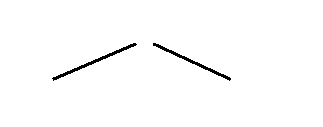
\includegraphics{expression.pdf}}
  \put(64.35,43.31){\fontsize{14.23}{17.07}\selectfont $+$}
  \put(5.67,8.73){\fontsize{14.23}{17.07}\selectfont $x_1* x_2$}
  \put(91.84,8.73){\fontsize{14.23}{17.07}\selectfont $y_1 * y_2$}
  \end{picture}
\else
\fi
\label{fig:expression}
\end{figure}
